% !TeX spellcheck = en_US
\documentclass[aspectratio=1610]{beamer}
\mode<presentation>
{
  \usetheme{Boadilla}
  \setbeamercovered{transparent}
  
  \definecolor{cobalt}{rgb}{0.0, 0.20, 0.50}
  
  \usecolortheme[named=cobalt]{structure}
  %\usecolortheme{lily}
  %\setbeamercolor{headline}{fg=cyan!80!black}
  % \setbeamercolor{frametitle}{bg=white}.
}

\makeatletter
\define@key{beamerframe}{wide}[10pt]{%
	\def\beamer@cramped{\itemsep #1\topsep0.5pt\relax}}
\makeatother
	

\usepackage[english]{babel}
\usepackage[utf8]{inputenc}
\usepackage{times}
\usepackage[T1]{fontenc}
\usepackage{array}
\usepackage{xcolor}
\usepackage{colortbl}
\usepackage{booktabs}

\title[Winter - Lecture 3] % (optional, use only with long paper titles)
{Macroeconomic Theory and Policy: Lecture  W3 (Ch.9)}

\author[University of Toronto] % (optional, use only with lots of authors)
{}
\date[] % (optional, should be abbreviation of conference name)

\begin{document}

\begin{frame}
  \titlepage
\end{frame}

\begin{frame}[wide]{What are You Going to Learn (Ch. 9)}
	\begin{itemize}
		\item How do we measures the economy’s performance in the short run? 
		\begin{itemize}
			\item Using the gap between actual GDP and potential GDP
		\end{itemize}
		\item How costly fluctuations in economic activity can be
		\item The rate of inflation tends to decline when the economy is in a recession
		\item A simple version of the short-run model that will help us understand these patterns
	\end{itemize}
\end{frame}

\begin{frame}[wide]{The Long Run, the Short Run, and Shocks}
	\begin{itemize}
		\item The long-run model describe how the economy behaves on average
			\begin{itemize}
				\item Solow model describes the steady state
				\item Romer model describes the long run growth rate
				\item The quantity theory of money sets long-run inflation
			\end{itemize}
		\item Potential output: amount of production if all inputs were utilized at their long-run sustainable levels
		\item At any given time, the economy is unlikely to exactly equal the long-run average
		\begin{itemize}
			\item The short run can be thought of as the length of time over which these deviations occur
			\item Deviations typically last for two years or so
		\end{itemize}
	\end{itemize}
\end{frame}

\begin{frame}[wide]{The Long Run, the Short Run, and Shocks}
	In the short-run model, 
	\begin{itemize}
		\item the current level of output and inflation are endogenous
		\item assume that the long run variables are given exogenous
		\begin{itemize}
			\item Potential output and the long-run rate of inflation are determined by the long-run model
			\item Since these variables are outside the short-run model, they are exogenous
		\end{itemize}
		\item current output can be deviated from potential output because of exogenous economic shocks
	\end{itemize}
\end{frame}

\begin{frame}[wide]{Trends and Fluctuations}
	\begin{itemize}
		\item Actual output is equal to the long-run trend plus short-run fluctuations
		\[\text{Actual Output} = \text{Long-run trend} + \text{short-run fluctuations}\]
		\[Y_t = \bar{Y}_t + \bar{Y}_t\times \tilde{Y}_t\]
		where
		\item[] \quad $\bar{Y}_t$ is the long-run trend (potential output) in level
		\item[] \quad $\tilde{Y}_t$ is the \textit{percentage} deviations from $\bar{Y}$ representing the short-run fluctuations
	\end{itemize}
\end{frame}

\begin{frame}[wide]{Short-Run Fluctuation}
	\begin{itemize}
		\item ``Detrended output" or short-run output is the difference in actual and potential output, expressed as a percentage of potential output:
		\[\tilde{Y}_t = \frac{Y_t -\bar{Y}_t}{\bar{Y}_t}\]
		\item Why do we express it in percentage?
		\begin{itemize}
			\item Suppose actual output falls short of potential output by \$100 million in a given year
			\item It depends on the overall size of the economy. In the US, \$100 million would be a much smaller fraction of GDP than is in Canada
			\item It is more informative to say actual output is, for example, 1 percent below potential
			\item This way, we can compare short-run measure across time and location
		\end{itemize}
	\end{itemize}
\end{frame}

\begin{frame}[wide]{Economic Fluctuations and Short-Run Output}
	\begin{itemize}
		\item Panel (a) shows actual and potential output
		\item Panel (b)	shows the implied short-run fluctuations
		\item When we remove the long-run trend associated with economic growth (potential output), what remains are the ups and downs of economic fluctuations
		\item When there is an expansion (recession), and the economy is booming (contracting), actual output is above (below) potential, and $\tilde{Y}$ is positive (negative)
		
	\end{itemize}
	\begin{figure}
		\centering
		\includegraphics[width=0.7\linewidth]{"Figures/fig 09_1"}
	\end{figure}
	
\end{frame}

\begin{frame}[wide]{Short-Run Output in the United States}
	\begin{itemize}
		\item Fluctuations in U.S. GDP:
		\begin{itemize}
			\item Difficult to see graphically over a long period of time if we plot it at level
			\item Have mostly been between + or –4\% since 1950
		\end{itemize}
		\item The Great Depression:
		\begin{itemize}
			\item Negative gap during the 1930s
			\item Actual output was well below potential output
			\item Take a long time to recover
		\end{itemize}
	\end{itemize}
\end{frame}

\begin{frame}[wide]{U.S. Real GDP, Actual and Potential}
	\begin{itemize}
		\item Because of the magnitude of economic growth, actual and potential output look quite similar on this time scale, even in ratio scale
		\item If we compute the difference between actual and potential output, the economic fluctuations become visible
	\end{itemize}
	\begin{figure}
		\centering
		\includegraphics[width=0.5\linewidth]{"Figures/fig 09_2"}
	\end{figure}
	
\end{frame}

\begin{frame}[wide]{U.S. Economic Fluctuations}
	\begin{itemize}
		\item A recession begins when actual output falls below potential and short-run output becomes negative
		\item A recession is usually end when short-run output starts to rise and become less negative before output returns to potential
	\end{itemize}
	\begin{figure}
		\centering
		\includegraphics[width=0.5\linewidth]{"Figures/fig 09_3"}
	\end{figure}
	
\end{frame}

\begin{frame}[wide]{Short Run}
	\begin{itemize}
		\item Typically, during a recession, output is below potential for approximately 2-4 years
		\begin{itemize}
			\item About 6 percent of GDP is foregone		
			\item Loss of about \$3,000 per person and between 1.5 million and 3 million jobs are lost
			
		\end{itemize}
		\item In addition, the decline in income is typically not spread evenly across the population
		\begin{itemize}
			\item To the extent that it's concentrated in particular regions, industries, and families, the costs to those affected can be even larger
			\item Unemployment rate rises by one or two percentage points
		\end{itemize}
		\item For a complete analysis of a cycle, we may also incorporate the benefits of a boom
	\end{itemize}
\end{frame}

\begin{frame}[wide]{Changes in U.S. Employment}
	\begin{itemize}
		\item Notice how severe the recent recession appears
		\item Total employment fell by more than 8.2 million jobs between Dec 2007 and Dec 2009: this is the largest decrease in employment in several decades
	\end{itemize}
	\begin{figure}
		\centering
		\includegraphics[width=0.6\linewidth]{"Figures/fig 09_4"}
	\end{figure}
	
\end{frame}



\begin{frame}[wide]{Scarring Effect}
	\begin{itemize}
		\item Below shows earning differences for workers who were jobless for over a year compared to those with similar income levels in the past five years by percentiles
		\item Left (right) panel shows the difference in average income after $k$ years  for the US (Canada)
	\end{itemize}
	\begin{figure}
		\centering
		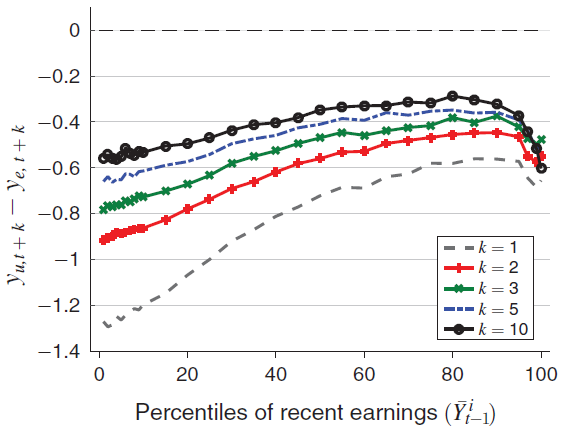
\includegraphics[width=0.45\linewidth]{Figures/scarring_1}
		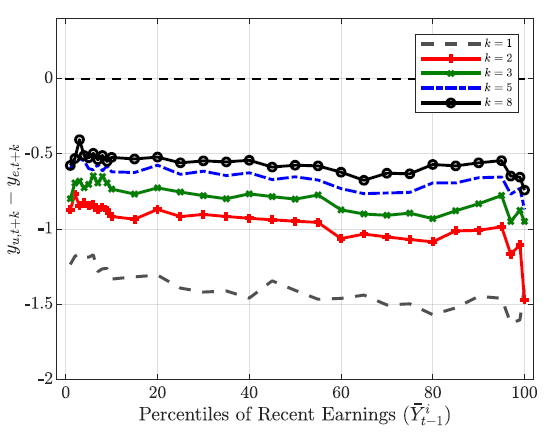
\includegraphics[width=0.45\linewidth]{Figures/scarring_2}
	\end{figure}
	\footnotetext{Source: Guvenen et.al (2017) and Kurnaz et.al (2024)}
\end{frame}

\begin{frame}[wide]{Scarring Effect}
	\begin{itemize}
		\item Canada experienced significantly higher income losses over the five years following post-unemployment
		\vspace{1mm}
		\begin{itemize}
			\item Losses in the US range between 40-60 log points, whereas Canadian losses range between 60-80 log points
		\end{itemize}
		\vspace{3mm}
		\item Losses in Canada demonstrate a weakly increasing trend over the income distribution, in contrast to the inverted U-shaped pattern observed in the US
		\vspace{3mm}
		\item The challenges of finding employment during a recession may lead to long-term negative effects for the unemployed beyond the initial 1-2 years of hardship
	\end{itemize}
\end{frame}

\begin{frame}[wide]{Long-term Unemployment in the US and Canada}
	\begin{itemize}
		\item Relative to the United States, Canada experiences a more modest increase in long-term unemployment.
		\item In both countries, long-term unemployment persists for a period exceeding 5 years
		\begin{itemize}
			\item Long-term unemployment is defined as being unemployed for roughly half a years
		\end{itemize}
	\end{itemize}
	\begin{figure}
		\centering
		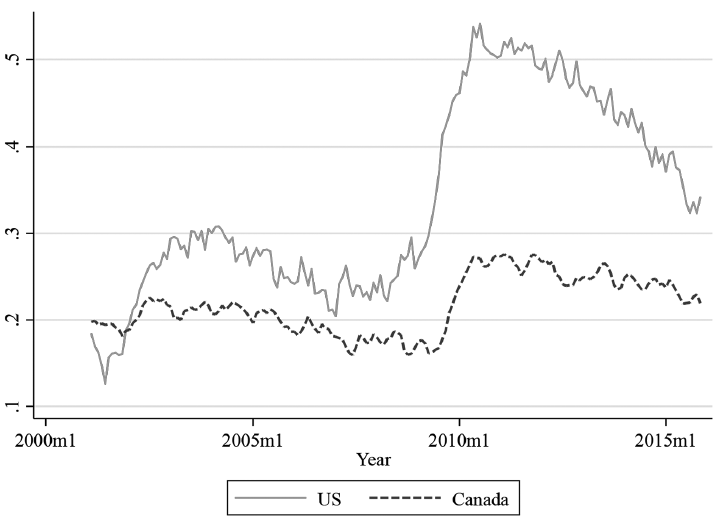
\includegraphics[width=0.5\linewidth]{Figures/scarring_3}
	\end{figure}
	\footnotetext{Source: Kroft et.al (2019)}
\end{frame}

\begin{frame}[wide]{Measuring Potential Output}
	\begin{itemize}
		\item There is no directly observable measure of potential output in an economy
		\item Ways to measure potential output:
		\begin{itemize}
			\item Fitting perfectly smooth trend passes through quarterly movements of real GDP
			\begin{itemize}
				\item e.g., Hodrick-Prescott filter, Baxter-King filter and more recently, Hamilton Filter
			\end{itemize}
			\item Take averages of the surrounding actual GDP numbers
			\begin{itemize}
				\item e.g., Moving average
			\end{itemize}
		\end{itemize}
		\item Annualized rate: rate of change that would apply if the growth rate persisted for an entire year
		\begin{itemize}
			\item If GDP increases by 1 percent over a single quarter, it will have grown at an annualized rate of 4 percent
		\end{itemize}		
	\end{itemize}
\end{frame}

\begin{frame}[wide]{Measuring Potential Output}
	\begin{itemize}
		\item Suppose we observe that GDP grew over the last quarter at an annualized rate of 5 percent
		\begin{itemize}
			\item How much of this increase in GDP reflects an increase in potential output?
			\item How much reflects a short-run fluctuation? 
			\item Is the economy now above potential, or has potential output grown rapidly?
		\end{itemize}
	\end{itemize}
\end{frame}

\begin{frame}[wide]{Measuring Potential Output}
	\begin{itemize}
		\item Economists consult a variety of indicators to answer this question. They examine
		\begin{itemize}
			\item data on how quickly the unemployed are finding jobs
			\item surveys revealing economic activity in particular industries
			\item demand by firms for new factories and equipment, and so on
		\end{itemize}
		\item If policymakers miscalculate whether the economy is in a recession or expansion, this can lead to unintended consequences, and sometimes exacerbate the effects of the business cycle
	\end{itemize}
\end{frame}



\begin{frame}[wide]{The Short-Run Model}
	The short-run model is based on three premises:
	\vspace{1mm}
	\begin{itemize}
		\item 	The economy is constantly being hit by shocks
		\vspace{1mm}
		\begin{itemize}
			\item Shocks: factors that cause fluctuations or even the potential output
			\begin{itemize}
				\item e.g., changes in oil prices, disruptions in financial markets, development of new technologies, natural disasters, etc
			\end{itemize}
		\end{itemize}
		\item Monetary and fiscal policies affect output
		\vspace{1mm}
		\begin{itemize}
			\item Policymakers can neutralize shocks to the economy
			\item e.g., BoC lowered the interest rate in the beginning of the pandemic 
		\end{itemize}
		\item There is a dynamic trade-off between output and inflation shown by the Phillips curve
	\end{itemize}
\end{frame}

\begin{frame}[wide]{The Phillips Curve (PC)}
	\begin{itemize}
		\item The Phillips curve (PC) shows
		\vspace{2mm}
		\begin{itemize}
			\item a positive relationship between the change in inflation and short-run output
			\item a boom increases inflation
			\item a recession decreases inflation
		\end{itemize}
		\vspace{4mm}
		\item Note we are interested in the change in inflation $\Delta \pi$ not the inflation rate itself $\pi$
		\vspace{2mm}
		\begin{itemize}
			\item Traditionally, the PC focus on the inflation rate 
			\item In 60s-70s, Milton Friedman (1968) and Edmund Phelps enhance the PC by introducing expectation to PC (more on that later)
		\end{itemize}
		
	\end{itemize}
\end{frame}

\begin{frame}[wide]{The Inflation Rate}
	\begin{itemize}
		\item The rate of inflation typically
		\begin{itemize}
			\item peaks at the start of a recession
			\item falls during the recession
		\end{itemize}
	\end{itemize}
	\begin{figure}
		\centering
		\includegraphics[width=0.7\linewidth]{"Figures/fig 09_5"}
	\end{figure}
\end{frame}

\begin{frame}[wide]{Works in a ``Cycle"}
	\begin{itemize}
		\item  Prices rise faster than the inflation rate for two reasons:
		\begin{itemize}
			\item In the economic boom, demand is higher, all firms are producing above potential, so higher prices follow
			\begin{itemize}
				\item the firms must raise wages, and perhaps delay maintenance on machines
				\item Firms must raise prices above the prevailing inflation rate to cover these costs
			\end{itemize}
		\begin{figure}
			\centering
			\includegraphics[width=0.5\linewidth]{"Figures/fig 09_7"}
		\end{figure}
		
		\end{itemize}
	\end{itemize}
\end{frame}

\begin{frame}[wide]{The Phillips Curve}
	\begin{itemize}
		\item The Phillips curve relates the change in the inflation rate to the amount of economic activity
		\begin{itemize}
			\item In a booming economy ($\tilde{Y}> 0$ ), inflation rises ($\Delta \pi >0$)
			\item In a slumping economy ($\tilde{Y}<0$), inflation falls($\Delta \pi <0$)
		\end{itemize}
	\end{itemize}
	\begin{figure}
		\centering
		\includegraphics[width=0.4\linewidth]{"Figures/fig 09_6"}
	\end{figure}
\end{frame}

\begin{frame}[wide]{Measuring the Phillips Curve}
	\begin{itemize}
		\item The positive sloped PC fit the data well for long time horizon
	\end{itemize}
	\begin{figure}
		\centering
		\includegraphics[width=0.7\linewidth]{"Figures/fig 09_8"}
	\end{figure}
\end{frame}

\begin{frame}[wide]{Measuring the Phillips Curve}
	\begin{itemize}
		\item Empirically, the slope is about 1/3
		\begin{itemize}
			\item If output exceeds potential by 3 percent, the inflation rate increases one percentage point
		\end{itemize}
		\vspace{2mm}
		\item In year 1979, inflation was high due to oil prices shock. The central bank decided to rise the interest rate to lower the inflation
		\vspace{1mm}
		\begin{itemize}
			\item As learn from the consumption/investment model, as interest increase, investment and consumption would fall. Thus, output will fall
		\end{itemize}
		\vspace{2mm}
		\item We can see that the points on the graph from 79-82, it is moving down along the PC
	\end{itemize}
\end{frame}

\begin{frame}[wide]{Okun’s Law: Output and Unemployment}
	\begin{itemize}
		\item Natural rate of unemployment: the rate of unemployment that exists in the long run, definded by $\bar{u}$
		\item Cyclical unemployment is the current unemployment minus the natural rate of unemployment
		\[u-\bar{u}\]
		\item In a recession, output is low and thus unemployment is high
		\item The relationship between this two variables is known as Okun’s law
		\[u-\bar{u}=-\frac{1}{2} \times \tilde{Y}\]
		\item Okun’s law says that for each percentage point that output is below potential, the unemployment rate exceeds its long-run level by half a percentage point
	\end{itemize}
\end{frame}

\begin{frame}[wide]{Okun’s Law for the U.S. Economy}
	\begin{itemize}
		\item Variable $\bar{u}$ is measured as the average rate in the surrounding period
		\item There is a tight, negative relationship between output and unemployment
	\end{itemize}
	\begin{figure}
		\centering
		\includegraphics[width=0.5\linewidth]{"Figures/fig 09_9"}
	\end{figure}
\end{frame}


\begin{frame}[wide]{Next Lecture}
	\begin{itemize}
		\item Next lecture will start Ch.11 
	\end{itemize}
\end{frame}

\end{document}